\chapter{Síntesis de Sonidos mediante Modelos Físicos}

\section{Introducción}
Se utilizó el modelo de Karplus-Strong para sintetizar el sonido de instrumentos de cuerda percutida u otros tipos de percusión. Este algoritmo, creado por Kevin Karplus y Alexander Strong en 1983 para sintetizar sonidos con pocos recursos y a tiempo real.

En este trabajo se analizaron el modelo básico para la síntesis de cuerdas percutidas y el modelo modificado para la síntesis de instrumentos de percusión.

\section{Modelo Conceptual}

En principio, el sistema se trata de un sistema linear excitado con una secuencia aleatoria de longitud finita $L$. El sistema consiste de una linea de retardo de $L$ muestras realimentadas a travéz de un filtro, tal como se ve en la figura \ref{fig:KS_model}.

\begin{figure}[ht]
    \centering
    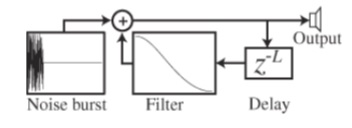
\includegraphics{res/ks_concept.jpg}
    \caption{Diagrama Conceptual del Modelo de Karplus-Strong}
    \label{fig:KS_model}
\end{figure}

La línea de retardo simula la cuerda, la cual los distintos armónicos de una nota recorren, se atenúan y decaen en el tiempo. En el modelo principal que se plantea en trabajo original de Kevin Karplus y Alex Strong, a la ausencia de algún filtro a la salida de la línea de retardo, la salida del sistema sería una repetición periódica de la señal entrante, lo que generaría un tono puro con una frecuencia de $f_s / L$, donde $f_s$ es la frecuencia de sampleo del sistema.

La modificación que inventa Alex Strong es promediar dos muestras consecutivas del sistema, generando un decaimiento lento de la amplitud en el tiempo. Matemáticamente, esta operación puede expresarse como en la expresión \eqref{eq:KS_avg}.

\begin{equation}
    Y_t = 0.5\times \left(Y_{t-L}+Y_{t-L-1}\right)
    \label{eq:KS_avg}
\end{equation}

Como consecuencia de esta modificación, la frecuencia del tono generado estará dada por la expresión \eqref{eq:KS_pitch}. Este tono tiene un sonido similar al de una cuerta percutida. Independientemente de las condiciones iniciales del sistema, el espectro decaerá hacia un tono puro, y eventualmente, a un valor constante (el silencio)

\begin{equation}
    f = \frac{f_s}{L+1/2}
    \label{eq:KS_pitch}
\end{equation}

Dado que para producir un sonido realista, se desea que el impulso inicial del sistema contenga una gran variedad de armónicos. Para ello existen distintas opciones. La primera es la propuesta por el mismo trabajo de Karplus-Strong: una señal aleatoria bi-nivel cuya expresión matemática está dada por \eqref{eq:2_level_random}, donde $A$ es la amplitud de la nota. Otras opciones para la excitación inicial con ruido es utilizar señales de ruido con distribución uniforme o gaussiana. Como estas muestras iniciales son repetidas periódicamente, no generarán ruido en el fondo.

\begin{equation}
    Y_t = 
    \begin{cases}
        +A  &   \text{probabilidad 0.5}\\
        -A  &   \text{probabilidad 0.5}
    \end{cases}
    \qquad  \text{para} -L\leq t \leq 0
    \label{eq:2_level_random}
\end{equation}

Finalemente, el modelo utilizado para simular la cuerda percutida será el de la figura \ref{fig:ks_original}. $x(n)$ será la señal inicial de entrada, por donde entrará la señal de ruido de longitud de muestras $L$.

\begin{figure}[ht]
    \centering
    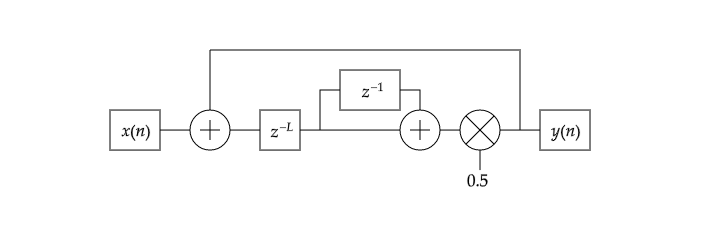
\includegraphics[width = \linewidth]{res/fig_ks.png}
    \caption{Modelo Original de Karplus Strong}
    \label{fig:ks_original}
\end{figure}

Modificando el modelo también es posible sintetizar instrumentos de percusión. Si se cambia el signo del promedio de las muestras aleatoriamente, como se ve en la figura \ref{fig:ks_drum}, matemáticamente tendrá un comportamiento expresado en \eqref{eq:ks_drum}. $b$ es llamado el factor de mezcla. Cuando $b=1$, el sistema se comporta normalmente y sigue simulando una cuerda. Cuando $b=0$, la señal es negada cada $L+0.5$ muestras, generando un sonido parecido a un arpa.

Finalemente, cuando $b=0.5$ se pierde el "tono" del sonido y este se asemejará más a un sonido percutido. $L$ ya no controla el tono, sino el tiempo de decaimiento. Dado que la naturaleza aleatoria ya se encuentra dentro del sistema, es suficiente con inicializar el sistema con una señal constante en lugar de utilizar ruido.

\begin{figure}[ht]
    \centering
    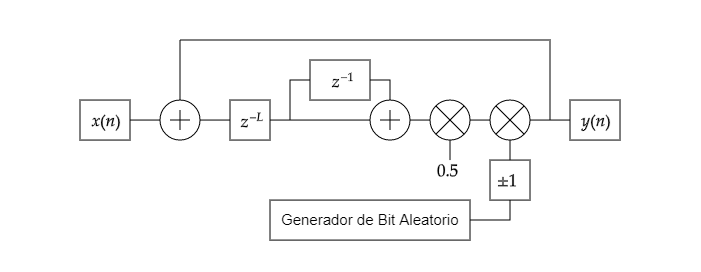
\includegraphics[width = \linewidth]{res/fig_ks_drum.png}
    \caption{Modelo Modificado de Karplus Strong para instrumentos de percusión}
    \label{fig:ks_drum}
\end{figure}

\begin{equation}
    Y_t = 
    \begin{cases}
        0.5\times \left(Y_{t-L}+Y_{t-L-1}\right) &   \text{probabilidad} \quad b \\
        -0.5\times \left(Y_{t-L}+Y_{t-L-1}\right) &   \text{probabilidad} \quad 1-b
    \end{cases}
    \label{eq:ks_drum}
\end{equation}

\section{Transferencia del Modelo}

Se calculó la función transferencia del modelo original de Karplus-Strong.

La transferencia del promedio está dada por

\begin{equation}
    H_a(z) = \frac{1+z^{-1}}{2}
\end{equation}

y la transferencia de la línea de retardo está dada por

\begin{equation}
    H_b(z) = z^{-L}
\end{equation}

Con esto, se obtiene que la transferencia de todo el sistema está dada por

\begin{equation}
    H(z) = \frac{1}{1- H_a(z) H_b(z)} = \frac{1/2\cdot (1+z^{-1})}{1-1/2\cdot z^{-L}(1+z^{-1})}= \frac{z+1}{2z^{L+1}-z-1}
    \label{eq:KS_H}
\end{equation}

A partir de la expresión \eqref{eq:KS_H} se puede calcular que existe un único cero en $z=-1$, que corresponde a la frecuencia de Nyquist $f_s/2$. Los polos pueden ser encontrados calculando las raíces de la expresión $2z^{L+1}-z-1 = 0$. Estas se pueden aproximar si la expresamos de la forma $2z^{L+1/2} = z^{1/2} + z^{-1/2}$. Reemplazando $z=a e^{j\omega}$ se obtiene:

\begin{equation}
    2 a^{L+1/2} e^{j\omega(L+1/2)} = a^{1/2}e^{j\omega/2} + a^{-1/2}e^{-j\omega/2}=\sqrt{a + a^{-1} + 2 \cos\omega } \cdot e^{j\theta}
\end{equation}

Analizando las partes imaginarias, se obtiene que

\begin{equation*}
    \sqrt{a + a^{-1} + 2 \cos\omega } \sin\theta = (a^{1/2} - a^{-1/2}) \sin\frac{\omega}{2}
\end{equation*}

Aproximando $e^{j\omega(L+1/2)} \approx 1$ se despeja que $\omega = 2 \pi n / (L+1/2)$. Aproximando $2 a^{p+1/2}\approx 2 cos(\omega/2)$ se puede despejar la constante del tiempo de caída del n-ésimo armónico, siendo
\begin{equation}
    a=\left[\cos\left( \frac{2 \pi n}{2L+1}\right)\right]^{1/(L+1/2)} = \left[\cos\left( \pi n \frac{f}{f_s}\right) \right]^{f/f_s}
    \label{eq:ks_pole_mod}
\end{equation}

Por lo tanto, los polos estarán ubicados en $z = a e^{j\omega}$ donde

\begin{equation*}
    a = \left[\cos\left( \frac{2 \pi n}{2L+1}\right)\right]^{1/(L+1/2)} \qquad \omega = \frac{2 \pi n}{L+1/2}
\end{equation*}

\begin{wrapfigure}{l}{0.5\textwidth}
    \centering
    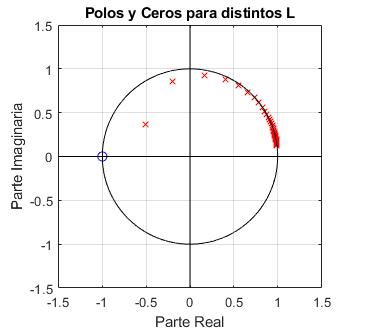
\includegraphics[width = 0.4\textwidth]{res/ks_zplane_orig.jpg}
    \caption{Polos y Ceros para distintos $L$}
    \label{fig:ks_zplane}
\end{wrapfigure}

En la figura \ref{fig:ks_zplane} se puede observar la distribución de los polos y ceros para distintos valores de $L\in[2,\infty)$, recorridos en sentido horario. Esto muestra que a valores pequeños de $L$, los polos se alejan de la aproximación asumida para su cálculo. Mientras tanto, el cero siempre está ubicado sobre $z=-1$.

La condición para la estabilidad es que, dado que este es un sistema causal y por lo tanto la región de convergencia no puede incluir a $z=0$, todos los polos deben estar ubicados dentro de la circunferencia de radio $|z|=1$. Tomando la expresión \eqref{eq:ks_pole_mod} se puede determinar que entonces

$\cos(x) < 1 \Rightarrow 0 < \pi n /(L+1/2) < \pi/2$

Dada la condición de Nyquist, se confirma entonces que este filtro será estable para cualquier longitud de retardo $L$.

\clearpage

\section{Afinamiento: selección de $L$}
A partir de la expresión \eqref{eq:KS_H}, la frecuencia de la nota generada estará dada por:
\begin{equation}
    f_1 = \frac{f_s}{P_a(z) + P_b(z)} = \frac{f_s}{L+1/2}
\end{equation}
donde $P_a(z)=1/2$ es la fase generada por el bloque promediador y $P_b(z)=L$ es la fase generada por el bloque de retardo. Dado que L es un número natural, las frecuencias fundamentales que se pueden generar con este modelo se verán cuantizadas. Sin embargo, como serán inversas a $L$ habrán diferencias en el error de la frecuencia generada dependiendo del tamaño de $L$. Para $L$ grande, esto no presentará un serio problema, ya que para dos $L$ consecutivos, las frecuencias estarán próximas unas a otras. Sin embargo, para $L$ chicos, las frecuencias estarán demasaido separadas.

Para solucionar este problema, es necesario, para altas frecuencias, poder cambiar el valor de la fase sin afectar la ganancia del filtro. Para esto se puede agregar un filtro pasa-todo de la forma \eqref{eq:KS_Hc}. Para que sea estable, $|C|<1$.

\begin{equation}
    H_c(z) = \frac{C + z^{-1}}{1+Cz^{-1}}\qquad P_c(z)\approx \frac{1-C}{1+C}
    \label{eq:KS_Hc}
\end{equation}

\begin{figure}[ht]
    \centering
    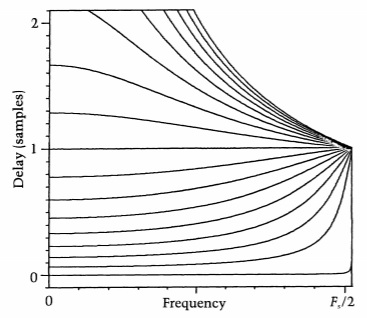
\includegraphics{res/allpass_phase.jpg}
    \caption{Retardo de Fase del filtro Pasa-Todo}
    \label{fig:KS_AllPass}
\end{figure}

Agregando este filto, la frecuencia de la nota generada estará dada por

\begin{equation*}
    f_1 = \frac{f_s}{P_a(z) + P_b(z) + P_c(z)}
\end{equation*}

En la figura \ref{fig:KS_AllPass} se puede observar cómo para distintos valores de $C$ la fase varía. Dado que la situación de retardo cero es difícil de obtener por errores de redondeo, es preferible que el retardo del filtro esté dado por $\varepsilon \leq P_c \leq 1+ \varepsilon$ para $\varepsilon$ chico. No es deseable superar el retardo de 1 dado que este deja de ser constante a altas frecuencias y retardos mayores.

Se puede calcular entonces la fase
\begin{equation*}
    L = \left\lfloor \frac{f_s}{f_1} - \frac{1}{2} - \varepsilon \right\rfloor
\end{equation*}
\begin{equation*}
    P_c = f_s/f_1 - N - 0.5
\end{equation*}

Para bajas frecuencias, se puede aproximar
\begin{equation*}
    C\approx\frac{1-P_c}{1+P_c}
\end{equation*}

De esta manera se puede afinar más precisamente la nota que se desea sintetizar.

\section{Posibles mejoras al modelo}
En el trabajo "Extensions of the Karplus Strong Algorithm" se detallan varias maneras en que se puede generar un sonido más convincente.

\subsection{Control del tiempo de decaimiento}
La primera mejora que presenta el trabajo es en el decaimiento de la señal. Esto se debe a que el tiempo de decaimiento de frecuencias bajas es demasiado distinta al de frecuencias altas.

Para acortar este tiempo, se puede agregar un factor de pérdida $\rho$ a la salida del promediador, de manera que el sistema quedaría caracterizado por:
\begin{equation*}
    y_n = x_n + \rho \frac{y_{n-N} + y_{n-(N+1)}}{2}
\end{equation*}
De esta manera, la amplitud de la envolvente de la señal será proporcional a:
\begin{equation*}
    \alpha_f(t,\rho)=|\rho \cos(\pi f T_s)|^{f_1 t} = |\rho|^{f_1 t} \alpha_f(t)
\end{equation*}
Y el tiempo de decaimiento quedará descripto por
\begin{equation*}
    \tau_1(\rho) = -\frac{1}{f_1 \ln|\rho \cos(\pi f_1 T_s)|}
\end{equation*}
Este método no sirve para alargar el decaimiento, dado que para mantener estabilidad $\rho \leq 1$.

Para ello se deberá implementar una modificación para el estiramiento de la nota. Esto se logra modificando la función de promedio por un promedio ponderado $(H_a)$ de manera que:
\begin{equation*}
    H_a(z,S) = (1-S) + Sz^{-1}
\end{equation*}
donde $S\in(0,1)$ es el factor de estiramiento.

La ganancia de este filtro estará dada por
\begin{equation*}
    G_a(f,S) = \sqrt{(1-S)^2+S^2+2S(1-S)\cos\omega T_s}
\end{equation*}
Cuando $S = 0.5$ se tiene el caso de la guitarra normal.

Sin embargo, agregar esta modificación altera la fase, de manera que ahora $P_a(f,S) \approx S$, el cálculo para generar la nota deberá ser $f = f_s / (N+S)$.

\section{Conclusión}
El modelo de Karplus Strong es uno fácil de implementar y altamente efectivo en la síntesis del sonido de una guitarra. Además, existen varias modificaciones menores al modelo que permiten agregar distintos efectos dinámicos y realismo a las notas, y generar timbres de otros instrumentos, como los de percusión.